The implementation of the alternative heuristics is based on the improvements
made by~\cite{devriendt2012symmetry} based on the MiniSAT SAT-solver.
In order to ease the testing procedure and overall usage of the solver, all heuristics
are implemented within the same program. One may choose one or multiple heuristics
by using command line parameters. Because of this feature it is possible to combine
multiple heuristics into a new heuristic.
While benchmarking we disabled the builtin heuristic that randomly chooses a literal from the heap,
such that our results are fully deterministic.
Further combinations of heuristics are not tested because this falls outside the scope
of this research.

We will analyze the results for each of the heuristics seperately and discuss for each of them both
hypothesis as formulated in section \ref{sec:Introduction}.
Beforehand we discuss some results that are observed for each of the measured heuristics.

\subsection{Generic Results}
	Firstly, it is observed that $SP^{REG}$ and $SP^{OPT}$ perform equally on all measured sets,
	except Urquhart.
	This conforms to our expectations, as the only difference between these implementations is the
	optimizing heuristic for inverting symmetries, and only the Urquhart set contains inverting
	symmetries in our selection of benchmarks.

	It is observed in the activity data that none of implementations, including $SP^{OPT}$,
	succeeds in increasing the number of active symmetries in the CHNL benchmark suite.

	The same is true for the Urquhart benchmarks.
	This however was to be expected, as it only contains inverting symmetries.
	The searcher therefor picks a branch literal (that is expected to keep more symmetries active),
	but during symmetry propagation, the weakly active symmetry would be made permanently inactive
	because it contains literals that invert under the symmetry.

	One might expect that SA would perform better under these circumstances.
	However, our implementation only performs \emph{unit propagation} during the lookahead, such
	that inverting symmetries are counted as active during the lookahead.

\subsection{SA Heuristic}
	From a theoretical perspective, SA was expected to have the most impact on the number of active
	symmetries during search, as it optimizes is very directly using a one iteration lookahead.
	This is reflected in the measured active symmetries.
	From all four heuristics, the SA heuristic is the one that performs best on this metric.

	The most prominent result is that it performs better (on the activity metric) than $SP^{OPT}$ in
	all but two battleship instances.
	Additionally, it keeps more symmetries active in the all of the shuffled pigeonhole benchmarks
	than $SP^{OPT}$.
	The first hypothesis is therefor true for the SA heuristic.

	When we look at the performance, however, there seems to be no correlation
	between the number of active symmetries and the number of decisions.
	This is made more clear by the scatter plot in figure \ref{fig:correlation}.
	If an increased amount of weakly active symmetries would have resulted in better performance in
	general and vice versa, than the scatter plot should have shown some increasing line.

	It is crucial to recall that SA chooses from the top five variables on the variable heap and
	does not alter anything else in the solver.
	The weakest conclusion that one can draw from this is that SA is not a better heuristic than the
	built-in VSIDS heuristic.
	The strongest conclusion would be to reject hypothesis 2, which we will discuss in
	\ref{ssec:falsification_hyp_2}.

	\begin{figure*}[!ht]
		\label{fig:correlation}
		\center
		\centerline{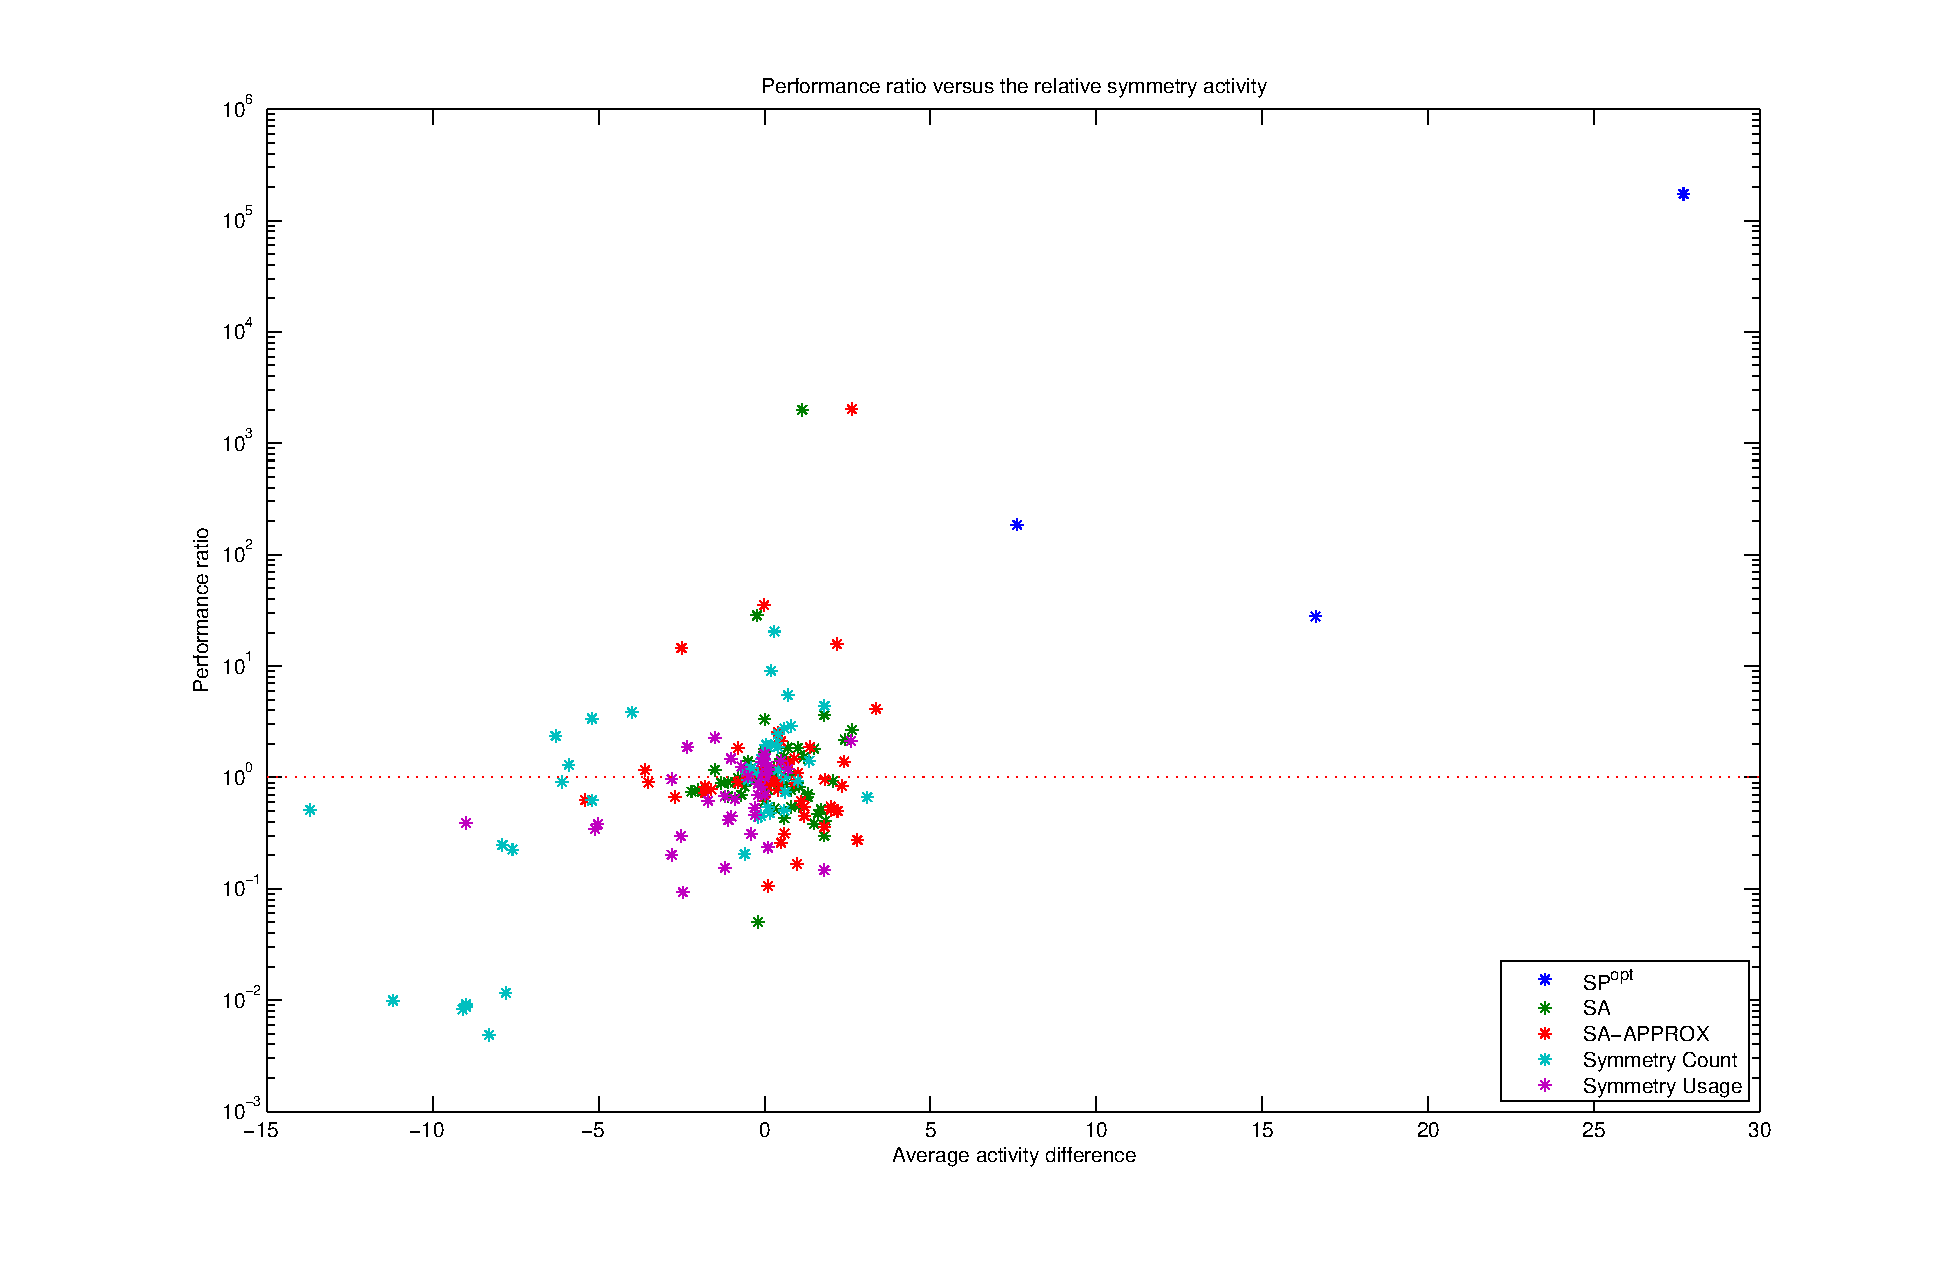
\includegraphics[width=1.2\textwidth]{results/scatterplot_activity.eps}}
		\caption{
			Correlation between number of active symmetries and number of decisions for all
			heuristics. Performance and activity measured relative to $SP^{REG}$.
		}
	\end{figure*}

\subsection{SU Heuristic}
	The symmetry usage statistic is performing very badly according to the activity metric.
	In

\subsection{On the Falsification of Hypothesis 2}
\label{ssec:falsification_hyp_2}
